% !TEX encoding = UTF-8
% !TEX TS-program = pdflatex
% !TEX root = ../tesi.tex

%**************************************************************
\chapter{Analisi dei requisiti}
\label{cap:analisi-requisiti}
Il presente capitolo ha come scopo fornire una descrizione completa e precisadi tutti i requisitiG individuati e dei casi d’uso ad alto livello riguardanti il progetto CS-Template.

\section{Casi d'uso}

Per lo studio dei casi di utilizzo del prodotto sono stati creati dei diagrammi.
I diagrammi dei casi d'uso (in inglese \emph{Use Case Diagram}) sono diagrammi di tipo \gls{uml} dedicati alla descrizione delle funzioni o servizi offerti da un sistema, così come sono percepiti e utilizzati dagli attori che interagiscono col sistema stesso.
Ogni caso d’uso è definito secondo la seguente struttura:
\begin{itemize}
	\item Nome: Il titolo del caso d’uso;
	\item Attori: Indica gli attori principali e secondari del caso d’uso. In tutto il contesto
	dell’applicazione gli utenti del sistema saranno così classificati:
	\begin{itemize}
		\item Agente: sono le persone che gestiscono ed elaborano le richieste dei clienti sulla piattaforma Zendesk;
		\item Zendesk Admin: utenti amministratori di Zendesk;
		 \item Amministratore: utente amministratore Nextep, che ha compito di gestire tutti le aziende che utilizzano l'applicazione CS-Template.
	\end{itemize}

	\item Descrizione: Riporta una breve descrizione del caso d’uso;
	\item Precondizione: Specifica le condizioni che sono identificate come vere prima
	del verificarsi degli eventi del caso d’uso;
	\item Postcondizione: Specifica le condizioni che sono identificate come vere dopo il
	verificarsi degli eventi del caso d’uso.

\end{itemize}

\subsection{ Casi d'uso pagina degli amministratori}
Questa è la pagina web il qui scopo princiaplae è quello di visualizzare la lista di tutti i clienti di Nextep che hanno l'applicazione CS-Template installata sulla propria piattaforma Zendesk. Inoltre permette di aggiungerne dei nuovi. L'accesso a questa pagina è garantita solo agli uenti amministratori di Nextep con le credenziali valide.
\begin{usecase}{1}{Login pagina amministratori}

	\usecaseactors{Utente generico}
	\usecasedesc{Caso d'uno descrive login alla pagina degli amministratori. }
	\usecasepre{L'utente non autenticato}
	\usecasepost{Il sistema riconosce l'utente amministratore}
		\begin{figure}[!h] 
		\centering 
		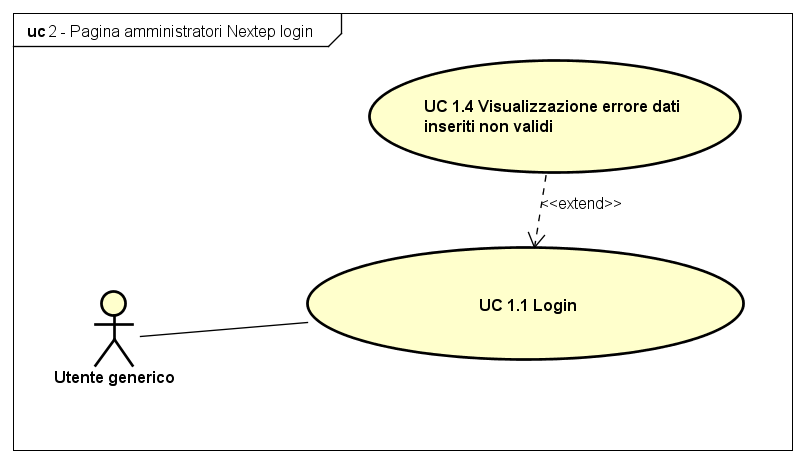
\includegraphics[width=1\columnwidth]{usecase/login} 
		\caption{UC 1 - pagina login}
	\end{figure}
\\ 
\\
\begin{usecase}{2}{Pagina degli amministratori}

\begin{usecase}{2}{Pagina degli amministratori}
	
	\usecaseactors{Nextep Admin}
	\usecasedesc{Caso d'uno descrive le funzionalità della pagina degli amministratori di Nextep. In questa pagina è possibile gestire tutti i clienti(aziende) di Nextep che utilizzano l'applicazione CS-Template}
	\usecasepre{Il sistema riconosce l'amministratore}
	\usecasepost{L’amministratore visualizza una lista di tutti i clienti(utilizzatori di CS-Template) registrati  nel  sistema,  visualizzando  per  ognuno  di  essi tutte le   informazioni  e un form per aggiungerne uno nuovoi}
	\begin{figure}[!h] 
		\centering 
		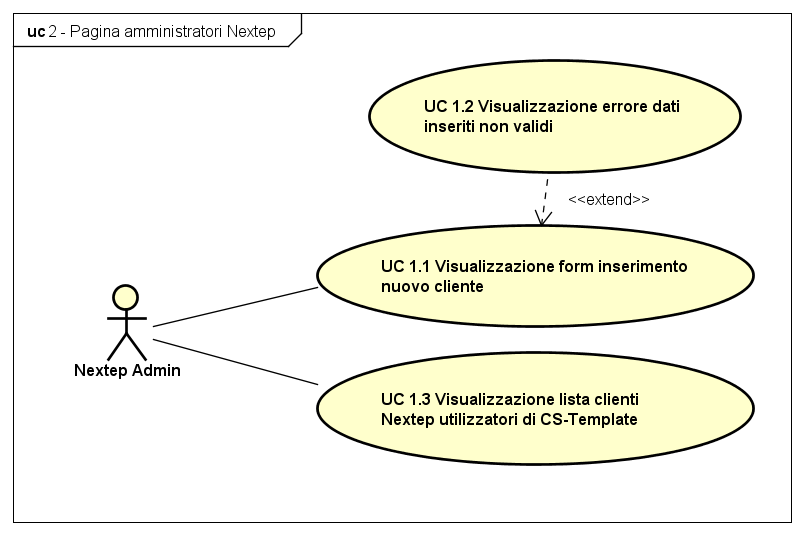
\includegraphics[width=1\columnwidth]{usecase/paginaAdmin} 
		\caption{UC 2 - funzionalità pagina admin}
	\end{figure}
\end{usecase}

\subsection{ Casi d'uso pagina contenente editor drag-and-drop}
Questa pagina web contiene l'editor drag-and-drop che verrà visualizzato successivamente nella piattaforma Zendesk in un iframe. In seguito è riportato un caso d'uso generico che descrive tutte le proprietà ad alto livello del editor.
\begin{usecase}{3}{Editor drag-and-drop}
	
	\usecaseactors{Utente Zendesk}
	\usecasedesc{Caso d'uso descrive tutte le funzionalità ad oalto livello che l'editor dovrà fornire}
	\usecasepre{L'utente Zendesk apre l'editor}
	\usecasepost{L'editor permette all'utente Zendesk di realizzare qualsiasi tipo di contentuto HTML e CSS}
	\begin{figure}[!h] 
		\centering 
		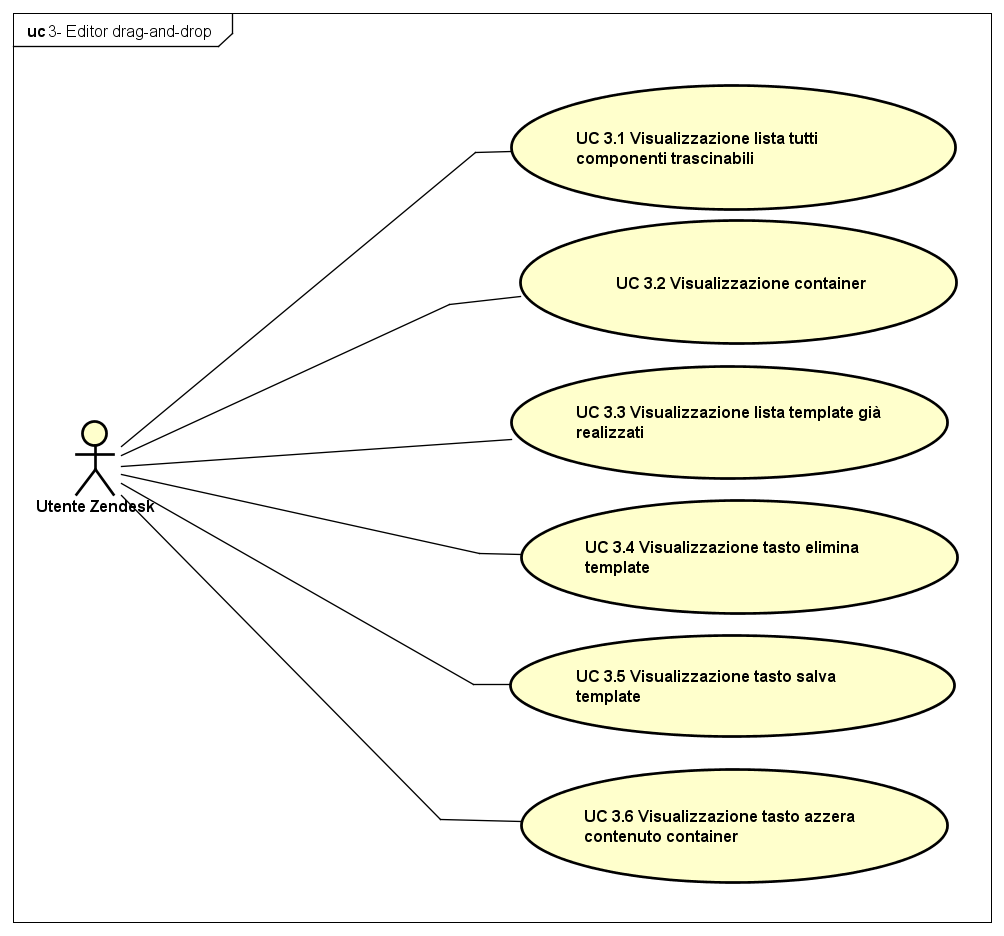
\includegraphics[width=1\columnwidth]{usecase/editor} 
		\caption{UC3 - pagina login}
	\end{figure}
	\\ 
	\\

\newpage
\section{Tracciamento dei requisiti}

Da un'attenta analisi dei requisiti e degli use case effettuata sul progetto è stata stilata la tabella che traccia i requisiti in rapporto agli use case.\\
Sono stati individuati diversi tipi di requisiti e si è quindi fatto utilizzo di un codice identificativo per distinguerli.\\
Il codice dei requisiti è così strutturato R(F/Q/V)(N/D/O) dove:
\begin{enumerate}
	\item[R =] requisito
    \item[F =] funzionale
    \item[Q =] qualitativo
    \item[V =] di vincolo
    \item[N =] obbligatorio (necessario)
    \item[D =] desiderabile
    \item[Z =] opzionale
\end{enumerate}
Nelle tabelle \ref{tab:requisiti-funzionali}, \ref{tab:requisiti-qualitativi} e \ref{tab:requisiti-vincolo} sono riassunti i requisiti e il loro tracciamento con gli use case delineati in fase di analisi.

\newpage

\begin{table}%
\caption{Tabella del tracciamento dei requisti funzionali}
\label{tab:requisiti-funzionali}
\begin{tabularx}{\textwidth}{lXl}
\hline\hline
\textbf{Requisito} & \textbf{Descrizione} & \textbf{Use Case}\\
\hline
RFN-1     & L'interfaccia permette di configurare il tipo di sonde del test & UC1 \\
\hline
\end{tabularx}
\end{table}%

\begin{table}%
\caption{Tabella del tracciamento dei requisiti qualitativi}
\label{tab:requisiti-qualitativi}
\begin{tabularx}{\textwidth}{lXl}
\hline\hline
\textbf{Requisito} & \textbf{Descrizione} & \textbf{Use Case}\\
\hline
RQD-1    & Le prestazioni del simulatore hardware deve garantire la giusta esecuzione dei test e non la generazione di falsi negativi & - \\
\hline
\end{tabularx}
\end{table}%

\begin{table}%
\caption{Tabella del tracciamento dei requisiti di vincolo}
\label{tab:requisiti-vincolo}
\begin{tabularx}{\textwidth}{lXl}
\hline\hline
\textbf{Requisito} & \textbf{Descrizione} & \textbf{Use Case}\\
\hline
RVO-1    & La libreria per l'esecuzione dei test automatici deve essere riutilizzabile & - \\
\hline
\end{tabularx}
\end{table}%